\documentclass[11pt,a4paper]{article}
\usepackage[utf8]{inputenc}
\usepackage[T1]{fontenc}
\usepackage{mathpazo}
\usepackage[scaled=0.9]{helvet}
\usepackage{amsmath,amssymb}
\usepackage[a4paper,top=2.5cm,bottom=2.5cm,left=2.4cm,right=2.4cm]{geometry}
\usepackage[table]{xcolor}
\usepackage{graphicx,booktabs,float,array,microtype}
\usepackage{titlesec,fancyhdr}
\usepackage[font=small,labelfont={bf,sf},textfont=it,labelsep=period]{caption}
\usepackage[colorlinks=true,linkcolor=azulsub,urlcolor=azulsub,citecolor=azulsub]{hyperref}

\definecolor{azultit}{RGB}{31,56,100}
\definecolor{azulsub}{RGB}{46,85,151}
\definecolor{cabecera}{RGB}{217,226,243}

% Este entorno no dispone de patrones de silabeo en español: se evita partir palabras
\hyphenpenalty=10000 \exhyphenpenalty=10000 \emergencystretch=3em \tolerance=2000

\renewcommand{\figurename}{Figura}
\renewcommand{\tablename}{Tabla}
\renewcommand{\contentsname}{Índice}
\captionsetup[table]{skip=4pt}

\renewcommand{\thesection}{\arabic{section}.}
\renewcommand{\thesubsection}{\arabic{section}.\arabic{subsection}.}
\titleformat{\section}{\Large\bfseries\color{azultit}}{\thesection}{0.5em}{}[\vspace{2pt}{\color{azulsub}\titlerule[0.8pt]}]
\titleformat{\subsection}{\large\bfseries\color{azulsub}}{\thesubsection}{0.5em}{}
\titlespacing*{\section}{0pt}{0pt}{12pt}
\titlespacing*{\subsection}{0pt}{12pt}{4pt}
\newcommand{\sectionbreak}{\clearpage}

\pagestyle{fancy}
\fancyhf{}
\fancyfoot[L]{\small\color{gray}2.º iMAT B — Grupo 4}
\fancyfoot[R]{\small\color{gray}Página \thepage}
\renewcommand{\headrulewidth}{0pt}

\newcommand{\cab}{\rowcolor{cabecera}}
\newcommand{\py}{\textsf{Python}}
\newcommand{\E}{\mathbb{E}}

\begin{document}

% =================== PORTADA ===================
\begin{titlepage}
\centering
\vspace*{1.5cm}

\includegraphics[width=0.55\linewidth]{figs/logo_comillas.png}\\[0.8cm]
{\large Grado en Ingeniería Matemática e Inteligencia Artificial (iMAT)}\\[2.5cm]
{\color{azultit}\rule{\linewidth}{1pt}}\\[0.6cm]
{\fontsize{30}{36}\selectfont\bfseries\color{azultit} MÉTODOS NUMÉRICOS}\\[0.4cm]
{\color{azultit}\rule{\linewidth}{1pt}}\\[1.4cm]
{\Large\itshape Proyecto}\\[0.4cm]
{\LARGE\bfseries Métodos tipo Monte Carlo}\\[2.2cm]
{\Large\bfseries 2.º iMAT B — Grupo 4}\\[0.2cm]
{\large\itshape Curso 2025 – 2026}\\[1.4cm]
{\large\bfseries\color{azulsub} Integrantes}\\[0.4cm]
Javier Martínez Montelongo\\[0.15cm]
Ignacio Mascarell Agúndez\\[0.15cm]
Juan Tabuyo Castell\\[0.15cm]
Jaime Tuesta de Simón\\[0.15cm]
Yago Vallarino Fernández-Cavada
\end{titlepage}

\pagenumbering{roman}
\begingroup
\renewcommand{\sectionbreak}{}
\tableofcontents
\endgroup
\clearpage
\pagenumbering{arabic}

% =================== 1 ===================
\section{Introducción}

La integración numérica tiene como objetivo aproximar el valor de una integral definida mediante un número finito de evaluaciones de la función integrando. Cuando no es posible calcular la integral de forma analítica, resulta imprescindible recurrir a métodos numéricos que proporcionen una estimación suficientemente precisa.

En los temas previos del curso se han estudiado métodos de tipo determinista, como las fórmulas de Newton–Côtes o las cuadraturas de Gauss. Estos métodos construyen la aproximación a partir de una selección fija y estructurada de puntos de evaluación y presentan una convergencia rápida en problemas de baja dimensión.

Existe, sin embargo, un enfoque alternativo basado en el uso de variables aleatorias. Los llamados \textbf{métodos tipo Monte Carlo} aproximan integrales mediante muestreo aleatorio, interpretando la integral como una esperanza matemática. Su convergencia es más lenta, del orden $\mathcal{O}(n^{-1/2})$, pero presentan una ventaja fundamental: su coste computacional no crece exponencialmente con la dimensión, a diferencia de los métodos basados en mallas regulares. Esto los hace imprescindibles en áreas como el \emph{Machine Learning} o la simulación de sistemas complejos.

El objetivo del presente proyecto es estudiar distintos métodos tipo Monte Carlo para aproximar integrales, analizar su variabilidad y su convergencia, explorar técnicas de reducción de varianza como el \emph{importance sampling} y comparar su comportamiento con el de métodos deterministas clásicos.

Todos los resultados numéricos de este informe se han obtenido con el notebook del proyecto ejecutado con la semilla aleatoria fija \texttt{0}, de modo que pueden reproducirse exactamente. Con otra semilla, los valores concretos varían ligeramente, aunque las conclusiones se mantienen.

% =================== 2 ===================
\section{Integración como valor esperado}

\subsection{Descripción}
Sea $f:[a,b]\to\mathbb{R}$ una función integrable y sea $X$ una variable aleatoria uniforme en $[a,b]$. Entonces se cumple la identidad
\begin{equation}
\int_a^b f(x)\,\mathrm{d}x \;=\; (b-a)\,\E[f(X)],
\end{equation}
lo que sugiere aproximar la integral mediante la media de evaluaciones de la función en puntos aleatorios. Sustituyendo la esperanza por la media muestral se obtiene el estimador
\begin{equation}
I_n \;=\; \frac{b-a}{n}\sum_{i=1}^{n} f(x_i) \;\approx\; \int_a^b f(x)\,\mathrm{d}x,
\end{equation}
donde los puntos $x_1,\dots,x_n$ se generan de forma aleatoria y uniforme en $[a,b]$.

\subsection{Implementación}
Se implementa en \py{} el estimador descrito y se aplica a tres funciones de prueba cuyo valor exacto es conocido, empleando $n = 10\,000$ muestras. Los resultados se recogen en la Tabla~\ref{tab:t1}.

\begin{table}[H]
\centering
\caption{Aproximación Monte Carlo uniforme para tres funciones de prueba ($n = 10\,000$).}\label{tab:t1}
\begin{tabular}{ccccc}
\toprule
\cab \textbf{Función} & \textbf{Intervalo} & \textbf{Valor exacto} & \textbf{Aprox. $I_n$} & \textbf{Error abs.}\\
\midrule
$x^2$ & $[0,1]$ & 0,33333 & 0,33033 & 0,00300\\
$\operatorname{sen}(x)$ & $[0,\pi]$ & 2,00000 & 1,98056 & 0,01944\\
$e^x$ & $[0,1]$ & 1,71828 & 1,71969 & 0,00140\\
\bottomrule
\end{tabular}
\end{table}

\subsection{Observaciones}
Los errores obtenidos son pequeños, entre $10^{-3}$ y $10^{-2}$ para $n = 10\,000$. No obstante, el resultado varía ligeramente en cada ejecución debido a la naturaleza estocástica del método; este comportamiento se analiza en detalle en la siguiente sección.

% =================== 3 ===================
\section{Variabilidad del método}

\subsection{Descripción}
A diferencia de los métodos deterministas, la salida de un algoritmo Monte Carlo depende de los números aleatorios generados, por lo que dos ejecuciones con el mismo número de muestras pueden producir resultados distintos. Es conveniente, por tanto, interpretar la salida del método como una variable aleatoria y estudiar su media y su varianza.

\subsection{Variabilidad entre ejecuciones}
Se realizan diez ejecuciones independientes del método para aproximar la integral de $f(x)=x^2$ en $[0,1]$ con $n = 10\,000$ muestras; los resultados se recogen en la Tabla~\ref{tab:t2}.

\begin{table}[H]
\centering
\caption{Diez ejecuciones independientes del método Monte Carlo uniforme ($f(x)=x^2$, $n = 10\,000$).}\label{tab:t2}
\begin{tabular}{cc}
\toprule
\cab \textbf{Ejecución} & \textbf{Aproximación $I_n$}\\
\midrule
1 & 0,3308676359493113\\
2 & 0,33299832384544553\\
3 & 0,33172436326380966\\
4 & 0,3336092892778177\\
5 & 0,334622223569936\\
6 & 0,334957128831692\\
7 & 0,33683213339104795\\
8 & 0,3379081338429348\\
9 & 0,33743878942983674\\
10 & 0,33436536939427214\\
\bottomrule
\end{tabular}
\end{table}

\begin{center}
\textbf{Media muestral:} 0,33453. \qquad \textbf{Varianza muestral:} $5{,}54099\cdot10^{-6}$.
\end{center}

\subsection{Media y varianza muestral}
La media y la varianza muestral insesgada se definen como
\begin{equation}
\bar I = \frac{1}{m}\sum_{j=1}^{m} I_n^{(j)}, \qquad S^2 = \frac{1}{m-1}\sum_{j=1}^{m}\left(I_n^{(j)}-\bar I\right)^2,
\end{equation}
donde el denominador $m-1$ garantiza que $S^2$ sea un estimador insesgado de la varianza. A medida que $n$ crece, la media debe converger al valor exacto y la varianza debe tender a cero. Con $m = 50$ repeticiones para cada valor de $n$ se obtienen los resultados de la Tabla~\ref{tab:t3}.

\begin{table}[H]
\centering
\caption{Media y varianza muestrales de 50 ejecuciones del método uniforme ($f(x)=x^2$).}\label{tab:t3}
\begin{tabular}{ccc}
\toprule
\cab $\boldsymbol{n}$ & \textbf{Media} & \textbf{Varianza}\\
\midrule
100 & 0,33447 & $6{,}55\cdot10^{-4}$\\
1\,000 & 0,33528 & $9{,}92\cdot10^{-5}$\\
10\,000 & 0,33328 & $1{,}00\cdot10^{-5}$\\
100\,000 & 0,33332 & $8{,}70\cdot10^{-7}$\\
\bottomrule
\end{tabular}
\end{table}

\subsection{Observaciones}
Para un $n$ fijo, las aproximaciones son distintas entre ejecuciones, pero una varianza baja basta para justificar la validez del método. Al iterar sobre distintos valores de $n$ se aprecia que la media converge al valor exacto y que la varianza decrece aproximadamente como $1/n$: multiplicar $n$ por 10 divide la varianza por un factor próximo a 10. Este comportamiento es compatible con el error típico de orden $\mathcal{O}(n^{-1/2})$.

% =================== 4 ===================
\section{Convergencia del método}

\subsection{Descripción}
Por la ley de los grandes números, el estimador $I_n$ converge al valor exacto de la integral cuando $n\to\infty$. El teorema central del límite garantiza además que el error típico decrece como $1/\sqrt{n}$, es decir, que el método Monte Carlo tiene orden de convergencia $\mathcal{O}(n^{-1/2})$. En esta sección se verifica esta afirmación de forma experimental.

\subsection{Error en función del número de muestras}
Se aproxima el valor de $\pi$ mediante la integral
\begin{equation}
\pi = \int_0^1 4\sqrt{1-x^2}\,\mathrm{d}x,
\end{equation}
para distintos valores de $n$. La Tabla~\ref{tab:t4} recoge las aproximaciones obtenidas (media de 30 ejecuciones para cada $n$) y sus respectivos errores.

\begin{table}[H]
\centering
\caption{Aproximación de $\pi$ mediante Monte Carlo uniforme para distintos valores de $n$.}\label{tab:t4}
\begin{tabular}{cccc}
\toprule
\cab $\boldsymbol{n}$ & \textbf{Aproximación} & \textbf{Error absoluto} & \textbf{Error relativo}\\
\midrule
10 & 3,1398426574 & 0,001750 & 0,0557\,\%\\
50 & 3,1185322266 & 0,023060 & 0,7340\,\%\\
100 & 3,1263963195 & 0,015196 & 0,4837\,\%\\
500 & 3,1403607739 & 0,001232 & 0,0392\,\%\\
1\,000 & 3,1454497711 & 0,003857 & 0,1228\,\%\\
5\,000 & 3,1419805810 & 0,000388 & 0,0123\,\%\\
10\,000 & 3,1434284161 & 0,001836 & 0,0584\,\%\\
50\,000 & 3,1416162048 & 0,000024 & 0,0007\,\%\\
100\,000 & 3,1416492394 & 0,000057 & 0,0018\,\%\\
500\,000 & 3,1417831716 & 0,000191 & 0,0061\,\%\\
1\,000\,000 & 3,1417630084 & 0,000170 & 0,0054\,\%\\
5\,000\,000 & 3,1416033547 & 0,000011 & 0,0003\,\%\\
\bottomrule
\end{tabular}
\end{table}

Representando el error en escala logarítmica frente al número de muestras, los puntos siguen de forma aproximada una recta de pendiente $-1/2$, como muestra la Figura~\ref{fig:f1}.

\begin{figure}[H]
\centering
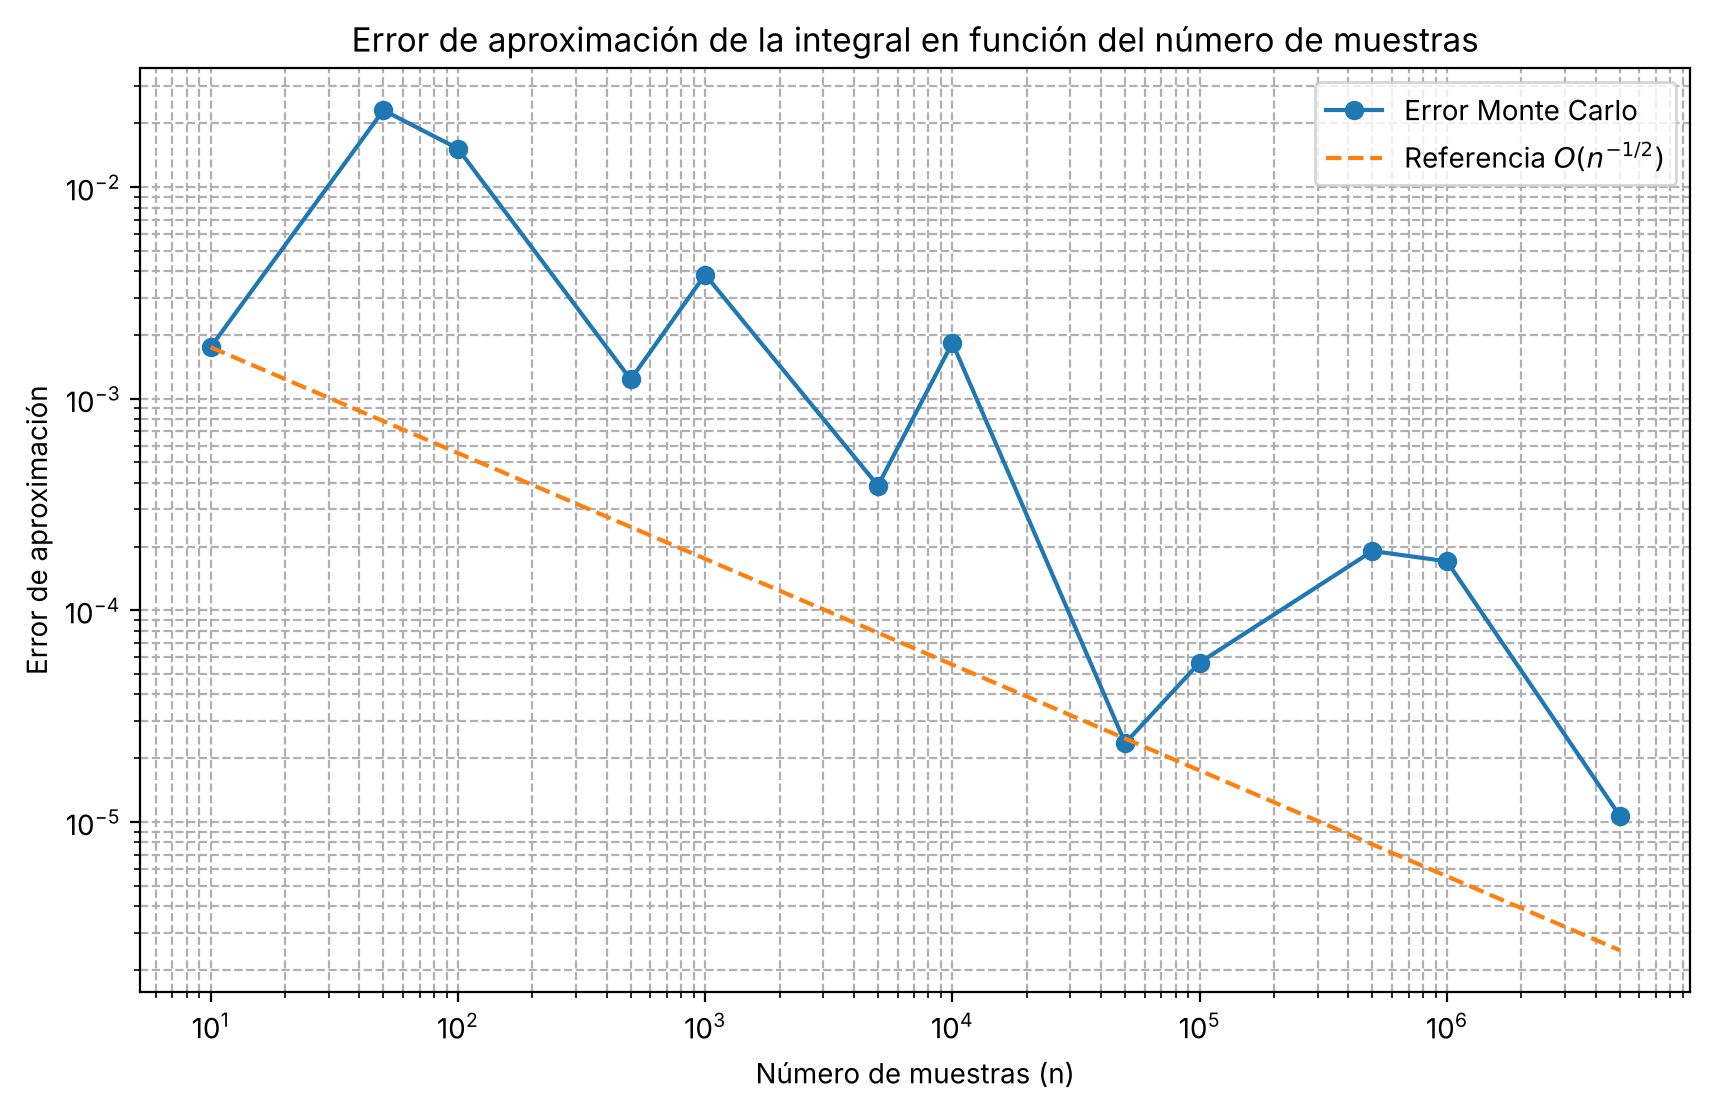
\includegraphics[width=0.8\linewidth]{figs/fig01_error_pi.png}
\caption{Error de aproximación de la integral en función del número de muestras $n$ (escala log–log). La línea discontinua representa la referencia teórica $\mathcal{O}(n^{-1/2})$, trazada desde el primer punto.}\label{fig:f1}
\end{figure}

\subsection{Estimación del orden de convergencia}
El orden de convergencia se estima a partir de la pendiente de los puntos $(\log n, \log|\text{error}|)$, que coincide con el exponente del orden. Calculando la pendiente media sobre 11 intervalos consecutivos (con una nueva serie de errores, promediada sobre 30 ejecuciones) se obtiene un valor de $\mathbf{-0{,}481}$, próximo al valor teórico esperado de $-0{,}5$.

\subsection{Observaciones}
Los resultados son consistentes con las hipótesis teóricas. La tendencia del error es muy similar a la recta de pendiente $-1/2$, con oscilaciones atribuibles al carácter estocástico del método, pese a haber promediado varias ejecuciones. La estimación directa de la pendiente confirma adicionalmente el orden de convergencia.

% =================== 5 ===================
\section{Método de aceptación–rechazo}

\subsection{Descripción}
Sea $f:[a,b]\to\mathbb{R}$ una función no negativa, y sea $M$ una cota superior tal que $0\le f(x)\le M$ para todo $x\in[a,b]$. La integral puede interpretarse entonces como el área de la región bajo la curva, contenida en el rectángulo $[a,b]\times[0,M]$. Si se generan $n$ puntos aleatorios uniformes en dicho rectángulo y una proporción $p$ de ellos cae bajo la gráfica, se tiene
\begin{equation}
\int_a^b f(x)\,\mathrm{d}x \;\approx\; p\cdot(b-a)\cdot M,
\end{equation}
donde un punto $(x_i,y_i)$ se acepta si cumple $y_i\le f(x_i)$ y se rechaza en caso contrario. La proporción $p$ se estima mediante el cociente entre propuestas aceptadas y propuestas totales.

\subsection{Implementación}
Se generan puntos aleatorios en el rectángulo $[a,b]\times[0,M]$ para las tres funciones analizadas en la sección~2, con $n = 100\,000$, y se comparan los resultados con los obtenidos mediante el método uniforme, recogidos en la Tabla~\ref{tab:t5}.

\begin{table}[H]
\centering
\caption{Comparación entre el método Monte Carlo uniforme y el método de aceptación–rechazo.}\label{tab:t5}
\begin{tabular}{ccccc}
\toprule
\cab \textbf{Función} & \textbf{Intervalo} & \textbf{Valor exacto} & \textbf{MC uniforme}\footnotemark & \textbf{Ac.–rechazo}\\
\midrule
$x^2$ & $[0,1]$ & 0,33333 & 0,33033 & 0,33319\\
$\operatorname{sen}(x)$ & $[0,\pi]$ & 2,00000 & 1,98056 & 2,00371\\
$e^x$ & $[0,1]$ & 1,71828 & 1,71969 & 1,71369\\
\bottomrule
\end{tabular}
\end{table}
\footnotetext{Los valores de la columna «MC uniforme» corresponden a las mismas ejecuciones que en la Tabla~\ref{tab:t1}.}

\subsection{Observaciones}
Los resultados del método de aceptación–rechazo son comparables a los del método uniforme. Su eficiencia depende crucialmente de lo ajustada que esté la cota $M$: si $M$ es mucho mayor que el máximo real de $f$, la proporción de puntos aceptados es pequeña y el método se vuelve ineficiente.

% =================== 6 ===================
\section{Importance sampling}

\subsection{Motivación}
El método Monte Carlo uniforme resulta ineficiente cuando la función integrando presenta picos estrechos y pronunciados. En tales situaciones, la mayor parte del valor de la integral proviene de regiones muy pequeñas del dominio, de manera que la mayoría de los puntos generados uniformemente caen en zonas donde la función toma valores despreciables. El resultado es una aproximación muy pobre, incluso con un número elevado de muestras.

Como ilustración, se aproxima la integral en $[-1,1]$ de una gaussiana concentrada, $f(x)=e^{-x^2/(2\sigma^2)}$ con $\sigma = 0{,}05$, con pico muy pronunciado en $x=0$. La aproximación obtenida con $n = 10\,000$ es 0,13039, siendo el valor exacto 0,12533. La integral sobre $\mathbb{R}$ coincide con $\sigma\sqrt{2\pi} = 0{,}12533$, y la diferencia con la integral sobre $[-1,1]$ es despreciable, ya que la función está concentrada en torno al origen.

\begin{figure}[H]
\centering
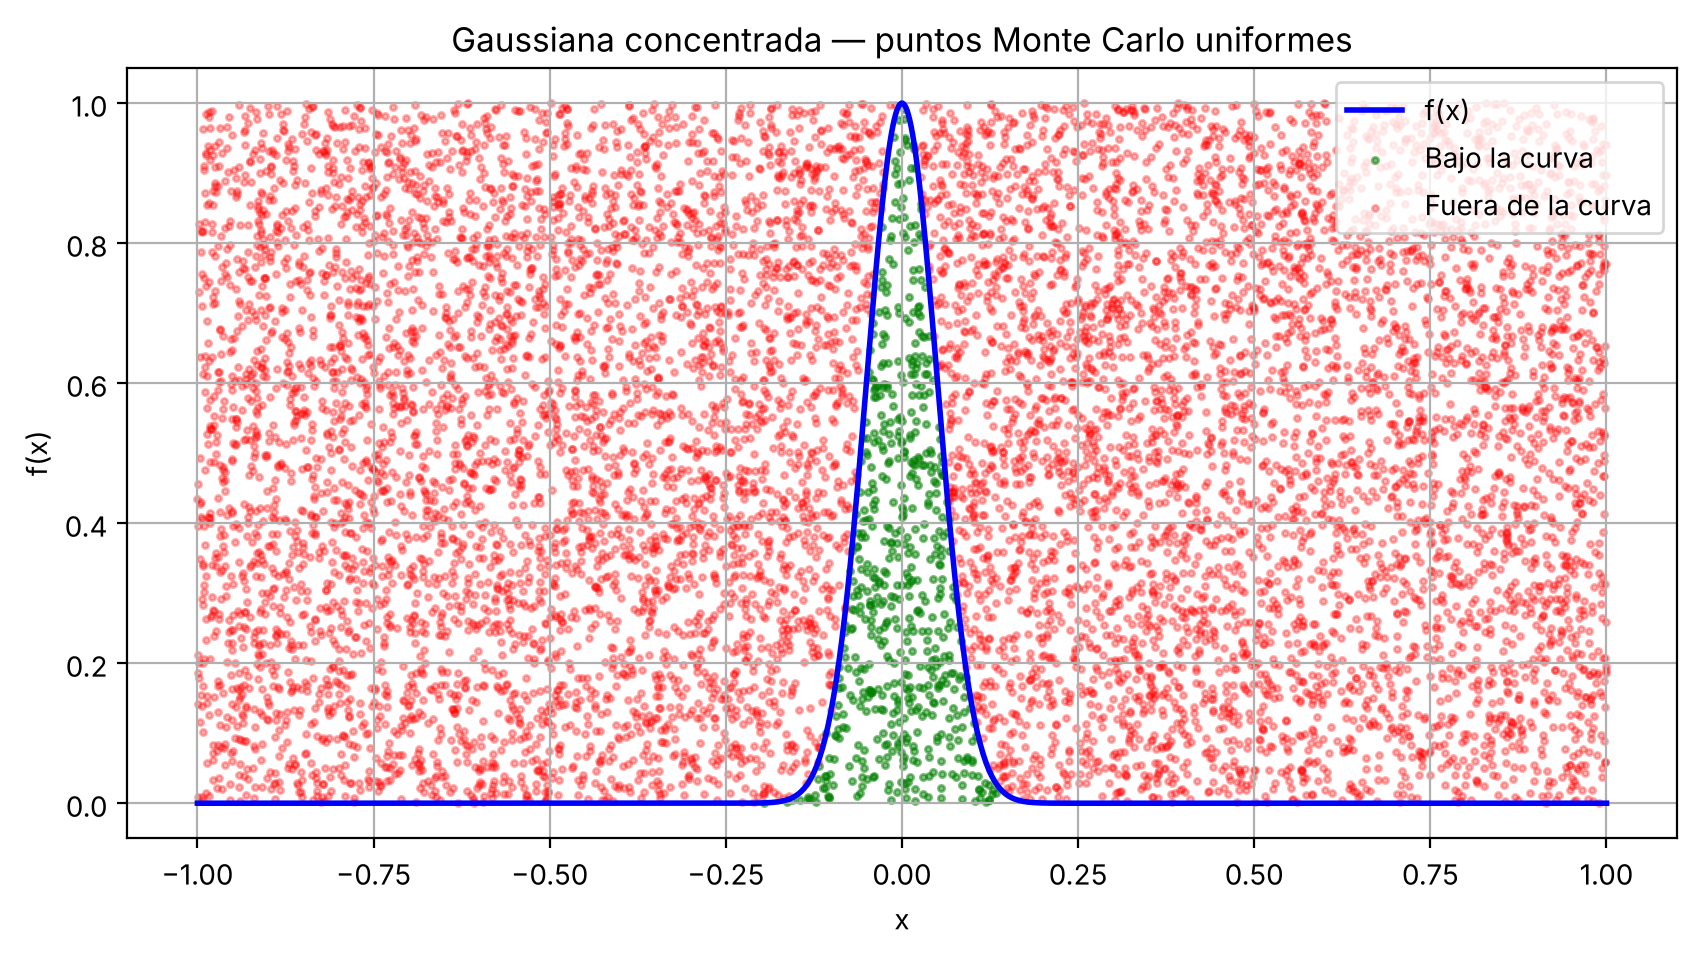
\includegraphics[width=0.8\linewidth]{figs/fig02_pico_muestreo.png}
\caption{Gaussiana concentrada: los puntos Monte Carlo uniformes (en rojo) caen mayoritariamente fuera de la región donde se concentra el área (en verde).}
\end{figure}

Se observa que la mayoría de los puntos caen fuera del pico, reflejo de la ineficiencia del muestreo uniforme. Repitiendo el experimento para diferentes valores de $n$, promediando 30 ejecuciones para reducir el ruido, se obtienen los resultados de la Tabla~\ref{tab:t6} y la Figura~\ref{fig:f3}.

\begin{table}[H]
\centering
\caption{Monte Carlo uniforme sobre una gaussiana concentrada: aproximación media y error medio sobre 30 ejecuciones.}\label{tab:t6}
\begin{tabular}{ccc}
\toprule
\cab $\boldsymbol{n}$ & \textbf{Aproximación media} & \textbf{Error medio}\\
\midrule
10 & 0,119847 & 0,105024\\
50 & 0,115476 & 0,056502\\
100 & 0,132772 & 0,032472\\
500 & 0,121615 & 0,015713\\
1\,000 & 0,124714 & 0,011528\\
5\,000 & 0,126558 & 0,004077\\
10\,000 & 0,125308 & 0,003290\\
50\,000 & 0,124614 & 0,001359\\
100\,000 & 0,125646 & 0,001243\\
500\,000 & 0,125305 & 0,000447\\
1\,000\,000 & 0,125216 & 0,000337\\
5\,000\,000 & 0,125363 & 0,000151\\
\bottomrule
\end{tabular}
\end{table}

\begin{figure}[H]
\centering
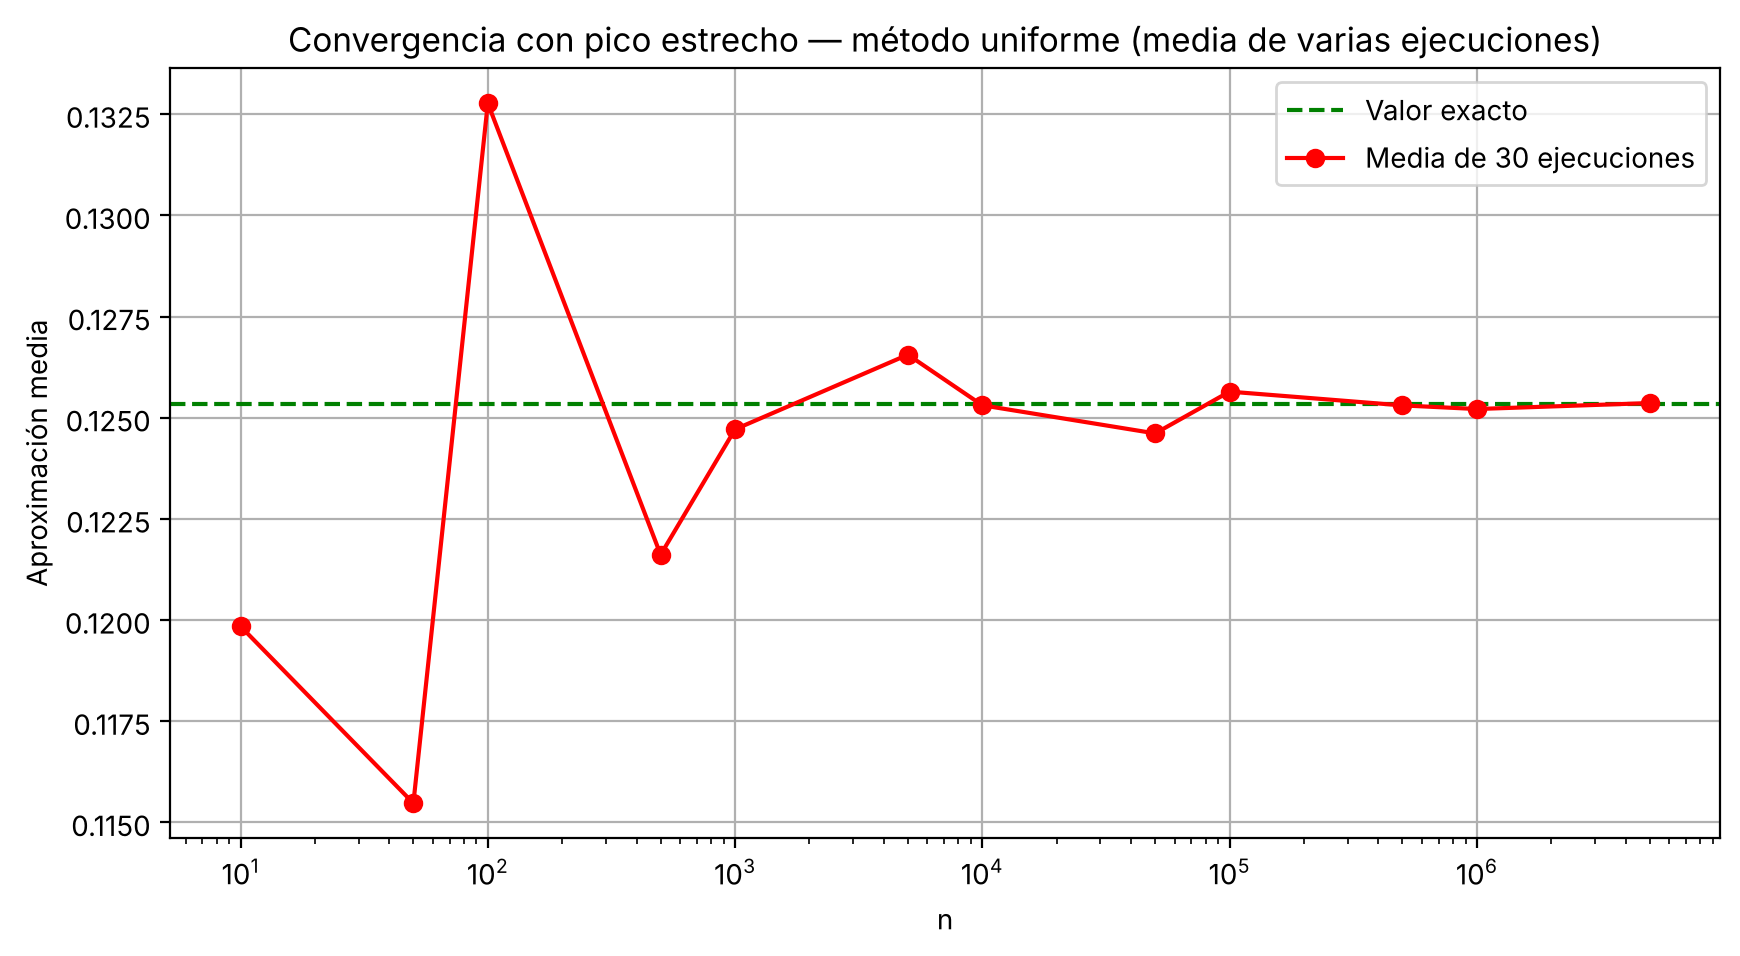
\includegraphics[width=0.8\linewidth]{figs/fig03_pico_convergencia.png}
\caption{Convergencia del método Monte Carlo uniforme para una gaussiana concentrada: media de 30 ejecuciones frente al valor exacto.}\label{fig:f3}
\end{figure}

Para valores pequeños de $n$, el error es muy elevado; sólo cuando $n$ crece notablemente la aproximación comienza a estabilizarse. Esto confirma que el método uniforme es muy ineficiente para funciones con picos.

\subsection{Método}
Sea $\rho(x)$ una densidad de probabilidad estrictamente positiva en $[a,b]$. La integral puede reescribirse como
\begin{equation}
\int_a^b f(x)\,\mathrm{d}x = \int_a^b \frac{f(x)}{\rho(x)}\,\rho(x)\,\mathrm{d}x \;\approx\; \frac{1}{n}\sum_{i=1}^{n}\frac{f(x_i)}{\rho(x_i)},
\end{equation}
donde los puntos $x_i$ se generan ahora según la densidad $\rho$. La idea es concentrar las muestras donde $f$ toma valores grandes eligiendo una densidad $\rho$ que se parezca a $f$ (salvo constante de normalización).

\subsection{Implementación}
En primer lugar, se aplica el método a $f(x)=x^2$ en $[0,1]$ utilizando la densidad $\rho(x)=2x$, que integra 1 en el intervalo y concentra masa hacia $x=1$. La aproximación obtenida es 0,33317 (exacto: 0,33333; error: 0,00017).

A continuación, se compara el comportamiento del método uniforme y del \emph{importance sampling} para la gaussiana concentrada anterior, empleando como $\rho$ una gaussiana proporcional a $f$. Los resultados se muestran en la Tabla~\ref{tab:t7} y la Figura~\ref{fig:f4}.

\begin{table}[H]
\centering
\caption{Comparación entre Monte Carlo uniforme e \emph{importance sampling} con $\rho\propto f$ para la gaussiana concentrada.}\label{tab:t7}
\begin{tabular}{ccccc}
\toprule
\cab $\boldsymbol{n}$ & \textbf{MC uniforme} & \textbf{Error uniforme} & \textbf{\emph{Imp. Sampling}} & \textbf{Error IS}\\
\midrule
10 & 0,138366 & 0,118422 & 0,125331 & $\approx 0$\\
50 & 0,129661 & 0,034119 & 0,125331 & $\approx 0$\\
100 & 0,121639 & 0,034393 & 0,125331 & $\approx 0$\\
500 & 0,123397 & 0,014052 & 0,125331 & $\approx 0$\\
1\,000 & 0,122292 & 0,011660 & 0,125331 & $\approx 0$\\
5\,000 & 0,124743 & 0,005188 & 0,125331 & $\approx 0$\\
10\,000 & 0,124331 & 0,003267 & 0,125331 & $\approx 0$\\
50\,000 & 0,125175 & 0,001173 & 0,125331 & $\approx 0$\\
100\,000 & 0,125365 & 0,000951 & 0,125331 & $\approx 0$\\
500\,000 & 0,125377 & 0,000457 & 0,125331 & $\approx 0$\\
\bottomrule
\end{tabular}
\end{table}

\begin{figure}[H]
\centering
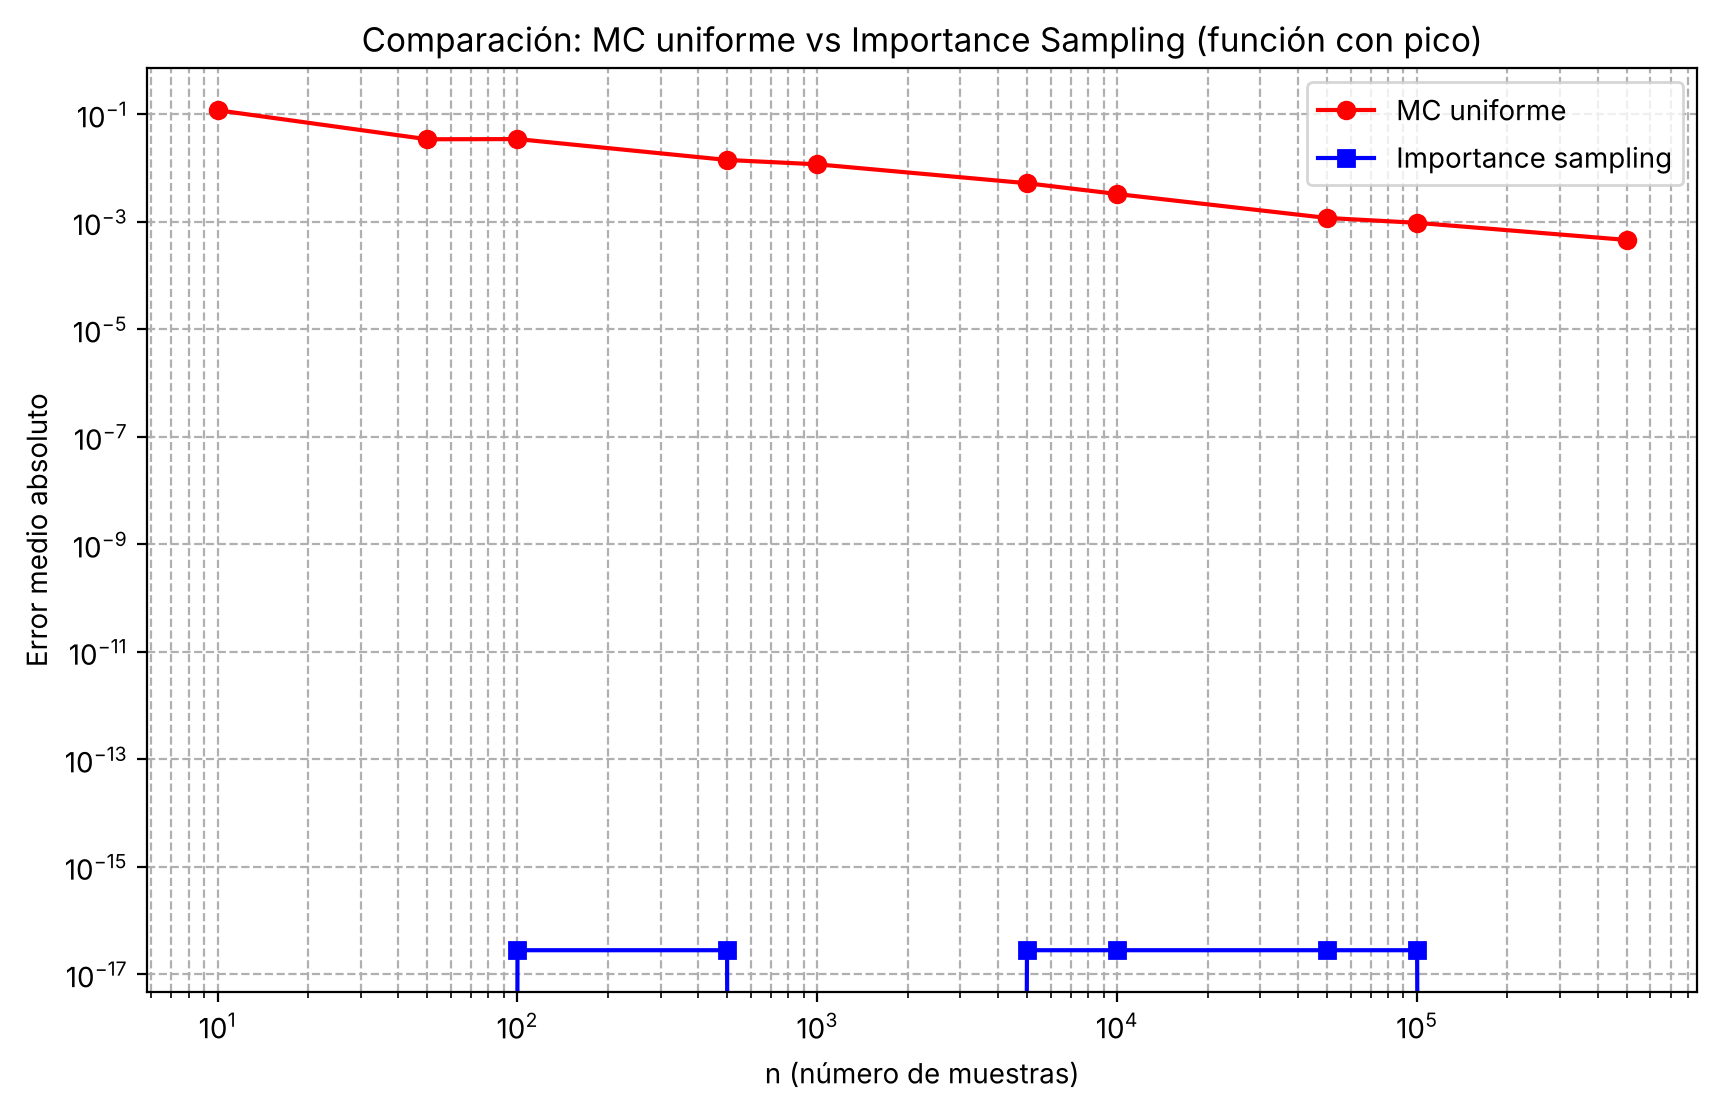
\includegraphics[width=0.8\linewidth]{figs/fig04_is_vs_uniforme.png}
\caption{Comparación log–log de MC uniforme e \emph{importance sampling} para una función con pico. Cuando $\rho\propto f$, el error del IS es prácticamente nulo.}\label{fig:f4}
\end{figure}

Se considera ahora la función $f(x)=1/(1+x^6)$ en $[-3,3]$, empleando como $\rho$ una gaussiana $\mathcal{N}(0,\sigma^2)$ truncada al intervalo, con $\sigma^2\in\{0{,}25;\ 1{,}0;\ 2{,}25;\ 4{,}0;\ 9{,}0\}$. El error medio se calcula sobre 30 ejecuciones con $n = 100\,000$ y se compara con el método uniforme.

\begin{center}
Valor exacto (cuadratura adaptativa): 2,09275004.\\
MC uniforme (30 ejecuciones): 2,092890, con error medio 0,007338.
\end{center}

\begin{table}[H]
\centering
\caption{\emph{Importance sampling} con distintas varianzas frente a MC uniforme para $f(x)=1/(1+x^6)$ en $[-3,3]$.}\label{tab:t8}
\begin{tabular}{ccccc}
\toprule
\cab $\boldsymbol{\sigma^2}$ & $\boldsymbol{\sigma}$ & \textbf{Aproximación IS} & \textbf{Error IS} & \textbf{Error MC uniforme}\\
\midrule
0,25 & 0,50 & 2,091851 & 0,005898 & 0,007338\\
1,00 & 1,00 & 2,092803 & 0,002384 & 0,007338\\
2,25 & 1,50 & 2,092839 & 0,004670 & 0,007338\\
4,00 & 2,00 & 2,092044 & 0,003687 & 0,007338\\
9,00 & 3,00 & 2,090628 & 0,005144 & 0,007338\\
\bottomrule
\end{tabular}
\end{table}

\begin{figure}[H]
\centering
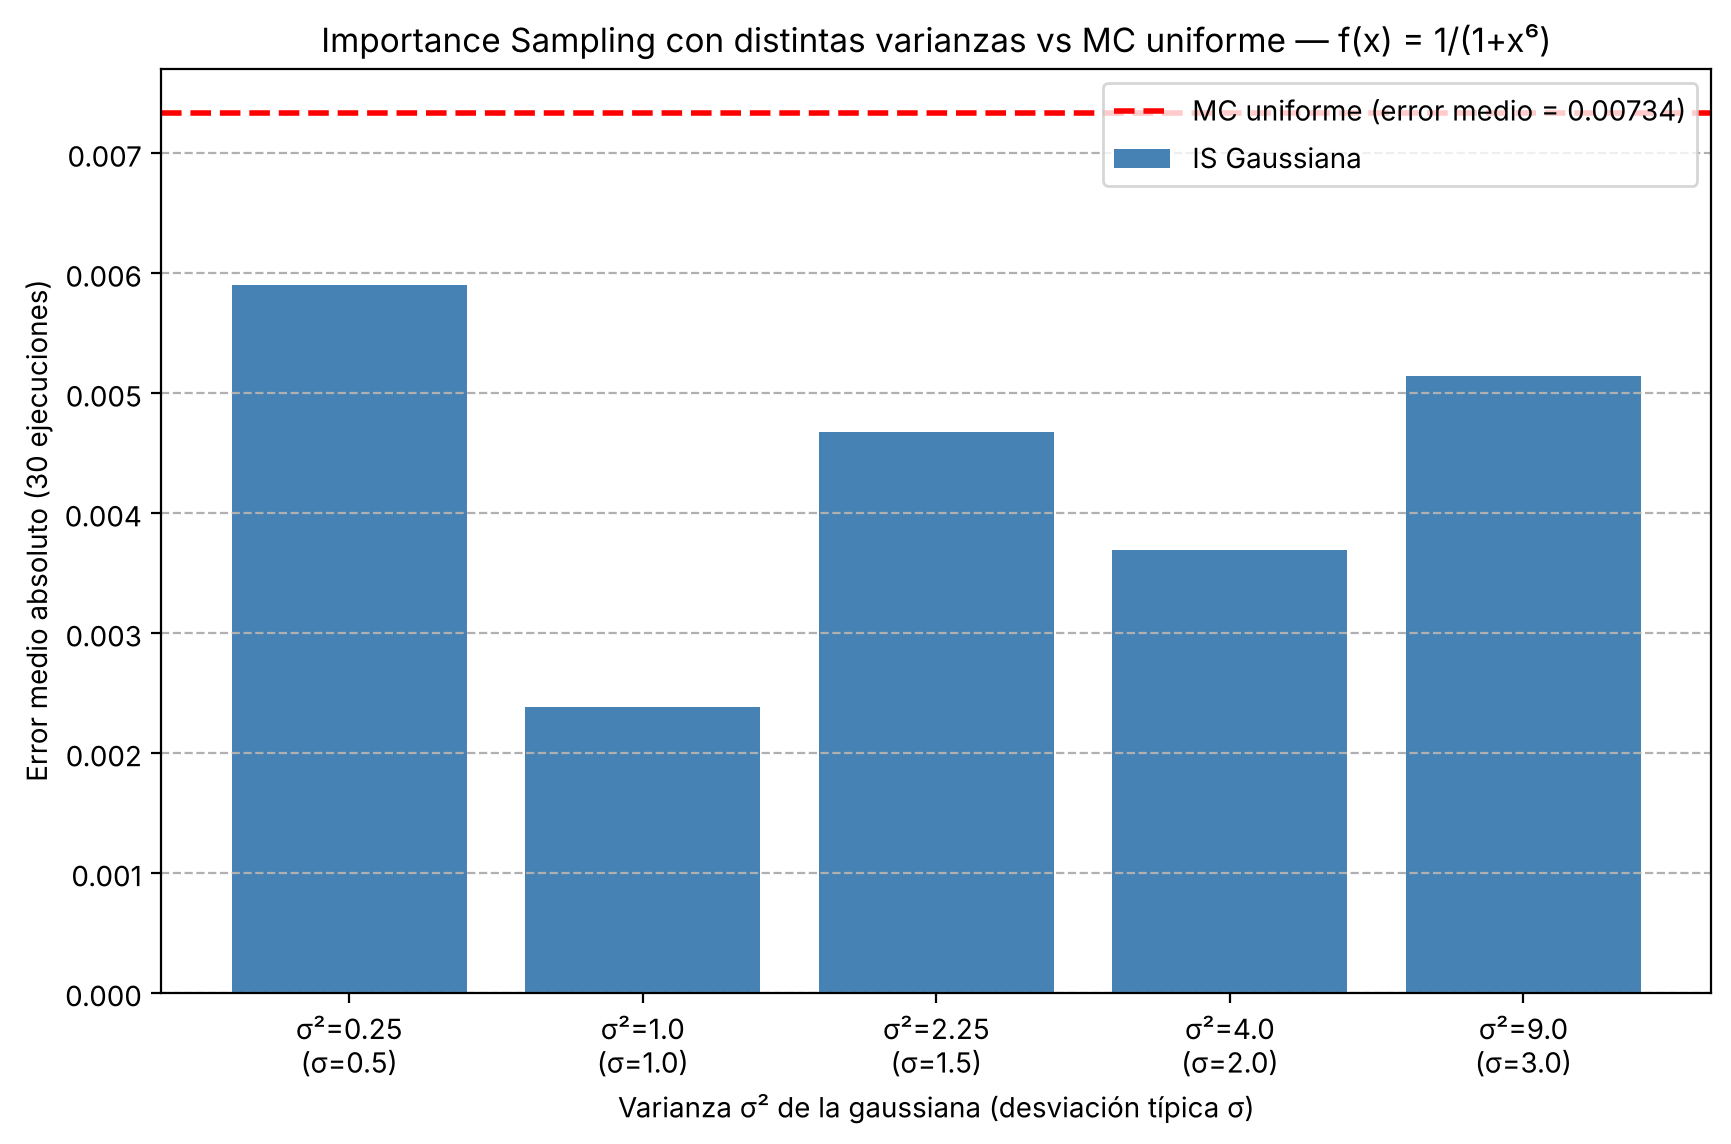
\includegraphics[width=0.8\linewidth]{figs/fig05_is_varianzas.png}
\caption{Error medio del \emph{importance sampling} para distintas varianzas de la gaussiana propuesta, comparado con la línea de referencia del MC uniforme.}
\end{figure}

La gaussiana con $\sigma^2\approx1$ ofrece los mejores resultados, ya que se adapta bien a la forma de $f$, que concentra la mayor parte de su área en torno al origen pero con colas moderadas. Una $\sigma^2$ demasiado pequeña concentra en exceso las muestras y desaprovecha las colas, mientras que una $\sigma^2$ demasiado grande dispersa las muestras y el método degenera hacia el comportamiento uniforme.

\subsection{Observaciones}
El \emph{importance sampling} reduce drásticamente el error del método uniforme cuando la densidad propuesta se adapta a la función integrando. En el caso ideal, $\rho\propto f$, el cociente $f/\rho$ es constante y la varianza del estimador se anula, de modo que la estimación es exacta. Este resultado, observado empíricamente en la Tabla~\ref{tab:t7}, constituye el fundamento teórico del método.

% =================== 7 ===================
\section{Comparación con métodos deterministas}

\subsection{Descripción}
En dimensión baja, los métodos deterministas clásicos presentan una convergencia notablemente más rápida que Monte Carlo. La regla del rectángulo, por ejemplo, alcanza un orden $\mathcal{O}(n^{-1})$ o superior, frente al orden $\mathcal{O}(n^{-1/2})$ del método Monte Carlo. En este apartado se comparan ambos métodos de forma empírica.

\subsection{Resultados}
Se evalúa la integral de $f(x)=e^x$ en $[0,1]$ mediante ambos métodos para distintos valores de $n$. La Tabla~\ref{tab:t9} recoge los errores y la Figura~\ref{fig:f6} los representa en escala log–log junto con las rectas de referencia teóricas.

\begin{table}[H]
\centering
\caption{Errores cometidos por Monte Carlo (media de 30 ejecuciones) y por la regla del rectángulo para la integral de $e^x$ en $[0,1]$.}\label{tab:t9}
\begin{tabular}{ccc}
\toprule
\cab $\boldsymbol{n}$ & \textbf{Error MC} & \textbf{Error regla del rectángulo}\\
\midrule
10 & 0,107257 & 0,084482\\
50 & 0,038859 & 0,017126\\
100 & 0,042064 & 0,008577\\
500 & 0,016345 & 0,001718\\
1\,000 & 0,011774 & 0,000859\\
5\,000 & 0,005116 & 0,000172\\
10\,000 & 0,004020 & 0,000086\\
50\,000 & 0,001851 & 0,000017\\
100\,000 & 0,001538 & 0,000009\\
500\,000 & 0,000675 & 0,000002\\
\bottomrule
\end{tabular}
\end{table}

\begin{figure}[H]
\centering
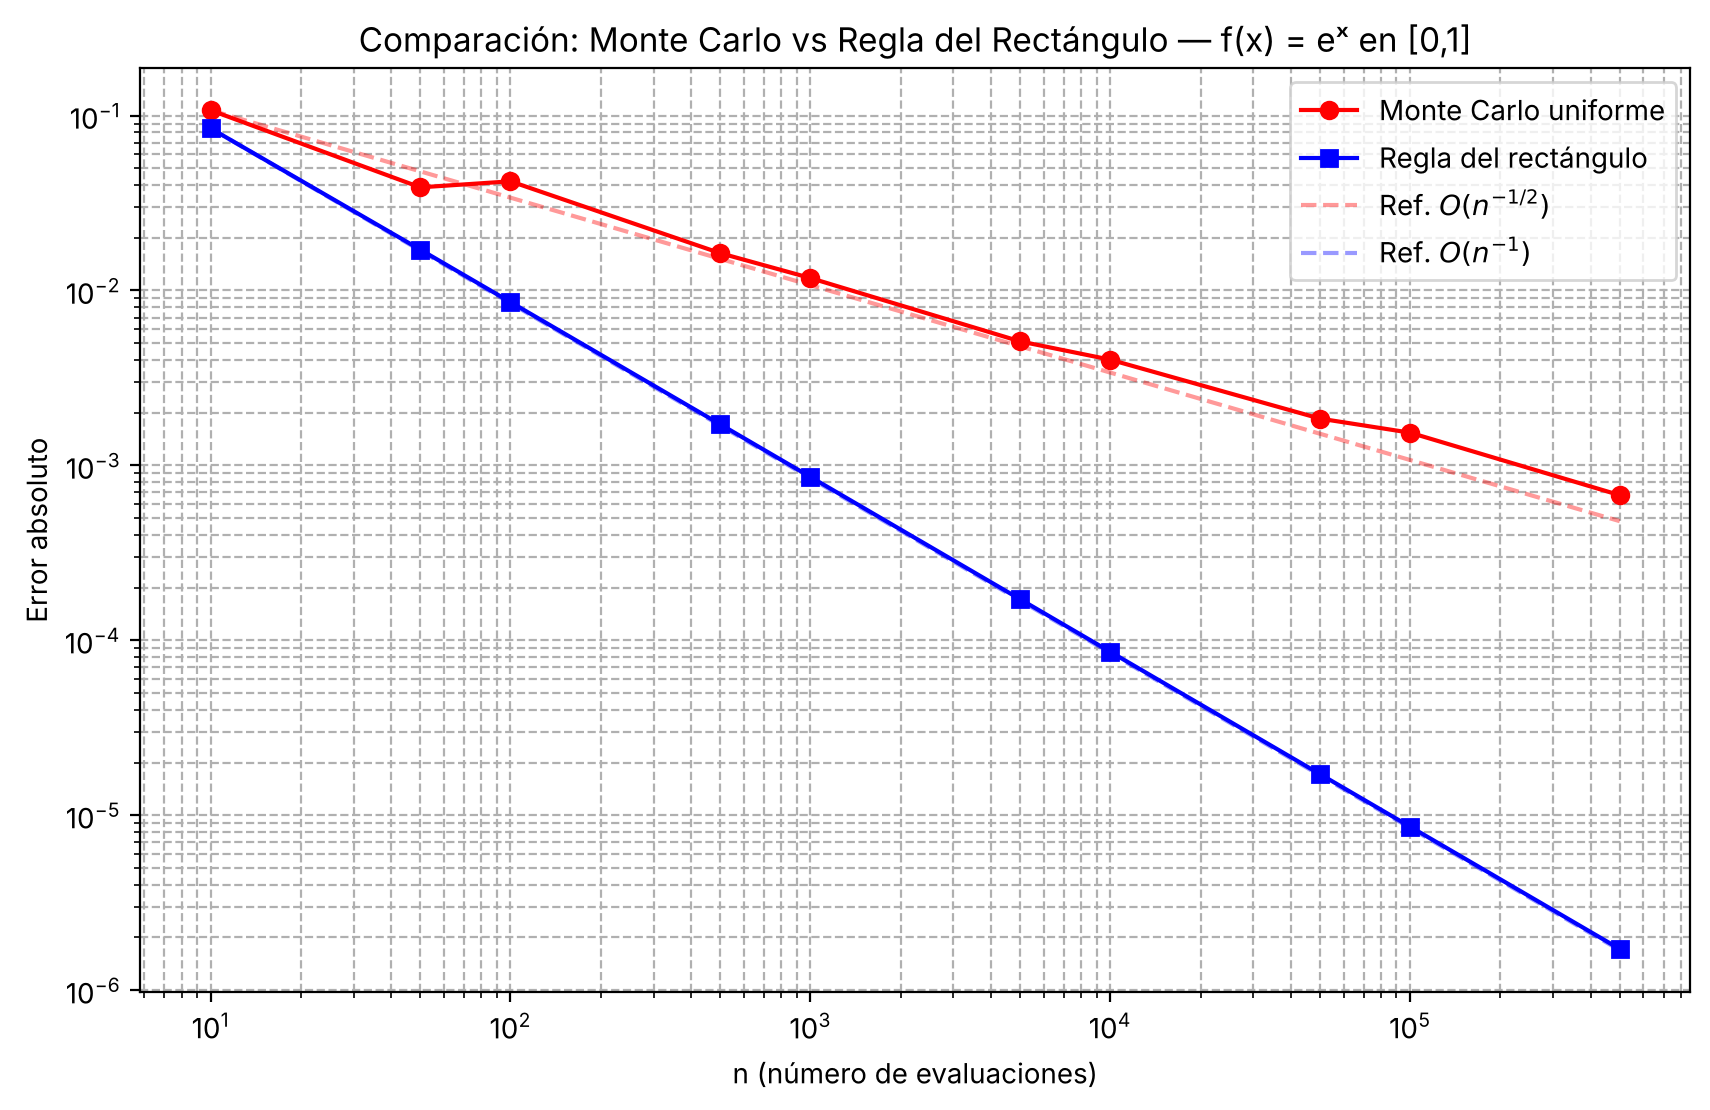
\includegraphics[width=0.8\linewidth]{figs/fig06_mc_vs_rectangulo.png}
\caption{Comparación log–log de Monte Carlo uniforme y regla del rectángulo para $f(x)=e^x$, junto con las referencias teóricas $\mathcal{O}(n^{-1/2})$ y $\mathcal{O}(n^{-1})$.}\label{fig:f6}
\end{figure}

\subsection{Observaciones}
La regla del rectángulo, con orden $\mathcal{O}(n^{-1})$, converge más rápidamente que Monte Carlo, cuyo orden es $\mathcal{O}(n^{-1/2})$. En problemas unidimensionales los métodos deterministas son, por tanto, claramente superiores. Sin embargo, como se verá en la siguiente sección, al aumentar la dimensión Monte Carlo conserva su orden de convergencia mientras que los métodos deterministas sufren la maldición de la dimensionalidad: al crecer la dimensión, el volumen del espacio aumenta exponencialmente y se requieren exponencialmente más puntos para mantener la misma densidad de muestreo.

% =================== 8 ===================
\section{Integración en dimensión superior}

\subsection{Descripción}
El método Monte Carlo se extiende de manera natural a integrales múltiples: basta con generar puntos uniformes en el dominio y promediar los valores de la función. En baja dimensión, los métodos deterministas basados en mallas siguen siendo más precisos, pero su coste computacional crece exponencialmente con la dimensión (maldición de la dimensionalidad). Por ello, en problemas de alta dimensión Monte Carlo resulta especialmente competitivo.

Si $\mathbf{x}_1,\dots,\mathbf{x}_n$ son puntos generados uniformemente en un dominio $D\subset\mathbb{R}^d$, la aproximación es
\begin{equation}
\int_D f(\mathbf{x})\,\mathrm{d}\mathbf{x} \;\approx\; \operatorname{vol}(D)\cdot\frac{1}{n}\sum_{i=1}^{n} f(\mathbf{x}_i),
\end{equation}
donde $\operatorname{vol}(D)$ denota el volumen del dominio. Esta formulación se extiende trivialmente a cualquier dimensión.

\subsection{Monte Carlo en dos dimensiones}
Se aplica el método a tres funciones de prueba en dominios rectangulares ($n = 100\,000$, 30 ejecuciones). La Tabla~\ref{tab:t10} recoge las aproximaciones obtenidas junto con los errores medios.

\begin{table}[H]
\centering
\caption{Monte Carlo uniforme sobre funciones bidimensionales en dominios rectangulares.}\label{tab:t10}
\begin{tabular}{ccccc}
\toprule
\cab \textbf{Función} & \textbf{Dominio} & \textbf{Aprox. MC} & \textbf{Valor exacto} & \textbf{Error medio}\\
\midrule
$x^2+y^2$ & $[0,1]\times[0,1]$ & 0,666951 & 0,666667 & 0,001300\\
$\operatorname{sen}(x)\cos(y)$ & $[0,\pi]\times[0,\pi/2]$ & 1,999777 & 2,000000 & 0,003625\\
$e^{-(x^2+y^2)}$ & $[-1,1]\times[-1,1]$ & 2,232533 & 2,230985 & 0,002291\\
\bottomrule
\end{tabular}
\end{table}

\begin{figure}[H]
\centering
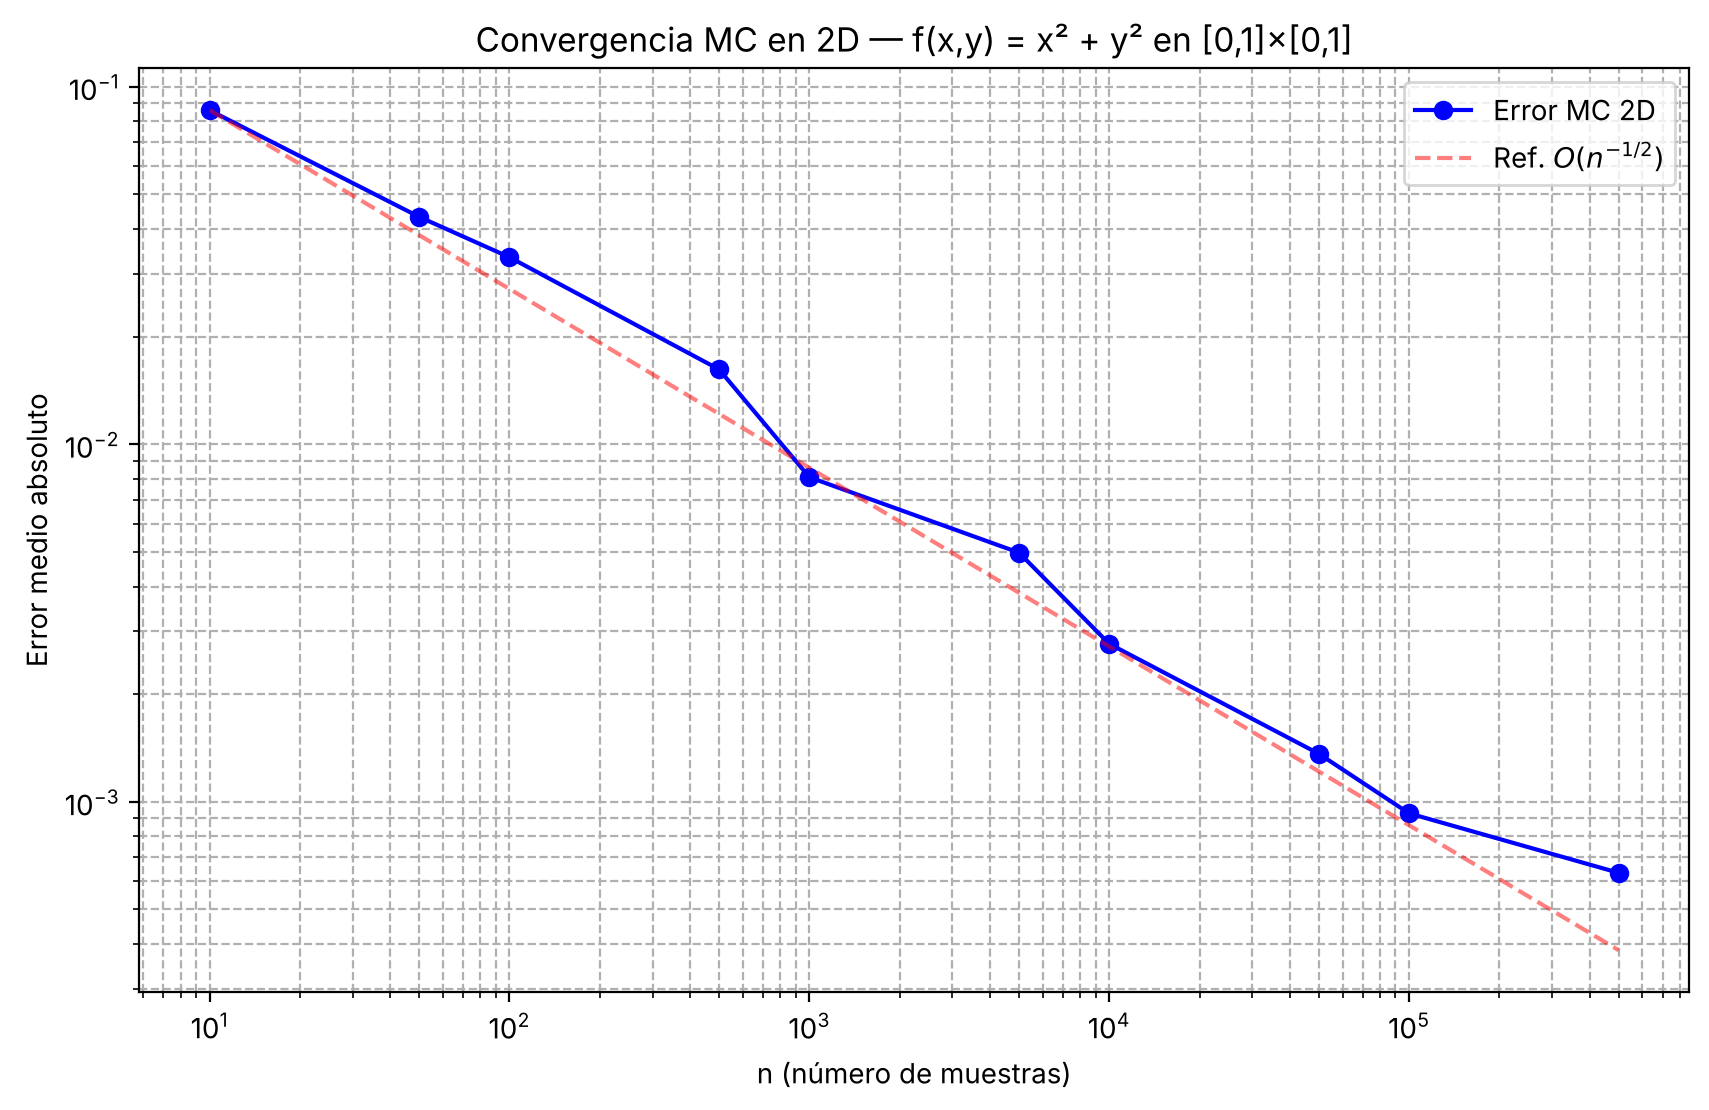
\includegraphics[width=0.8\linewidth]{figs/fig07_mc2d_convergencia.png}
\caption{Convergencia del método Monte Carlo en 2D para $f(x,y)=x^2+y^2$ en $[0,1]\times[0,1]$. La pendiente en log–log se mantiene próxima a $\mathcal{O}(n^{-1/2})$.}
\end{figure}

Con esto se comprueba que el orden de convergencia se mantiene en $\mathcal{O}(n^{-1/2})$, igual que en una dimensión. Esta invariancia frente a la dimensión es una de las mayores ventajas del método.

El método se extiende además a dominios no rectangulares mediante un criterio de aceptación. Se consideran dos funciones sobre el disco unitario: $f(x,y)=1$ y $f(x,y)=x^2+y^2$. Los puntos se generan uniformemente en $[-1,1]\times[-1,1]$ y se aceptan únicamente aquellos que satisfacen $x^2+y^2\le1$. Con $n = 200\,000$ puntos y promediando 30 aproximaciones, se obtienen los resultados de la Tabla~\ref{tab:t11}.

\begin{table}[H]
\centering
\caption{Monte Carlo con aceptación–rechazo sobre el disco unitario ($n = 200\,000$, 30 repeticiones).}\label{tab:t11}
\begin{tabular}{cccc}
\toprule
\cab \textbf{Función} & \textbf{Aprox. MC} & \textbf{Valor exacto} & \textbf{Error}\\
\midrule
$f=1$ (área del disco) & 3,141593 & 3,141593 & 0,000000\\
$f=x^2+y^2$ & 1,571295 & 1,570796 & 0,000499\\
\bottomrule
\end{tabular}
\end{table}

\begin{figure}[H]
\centering
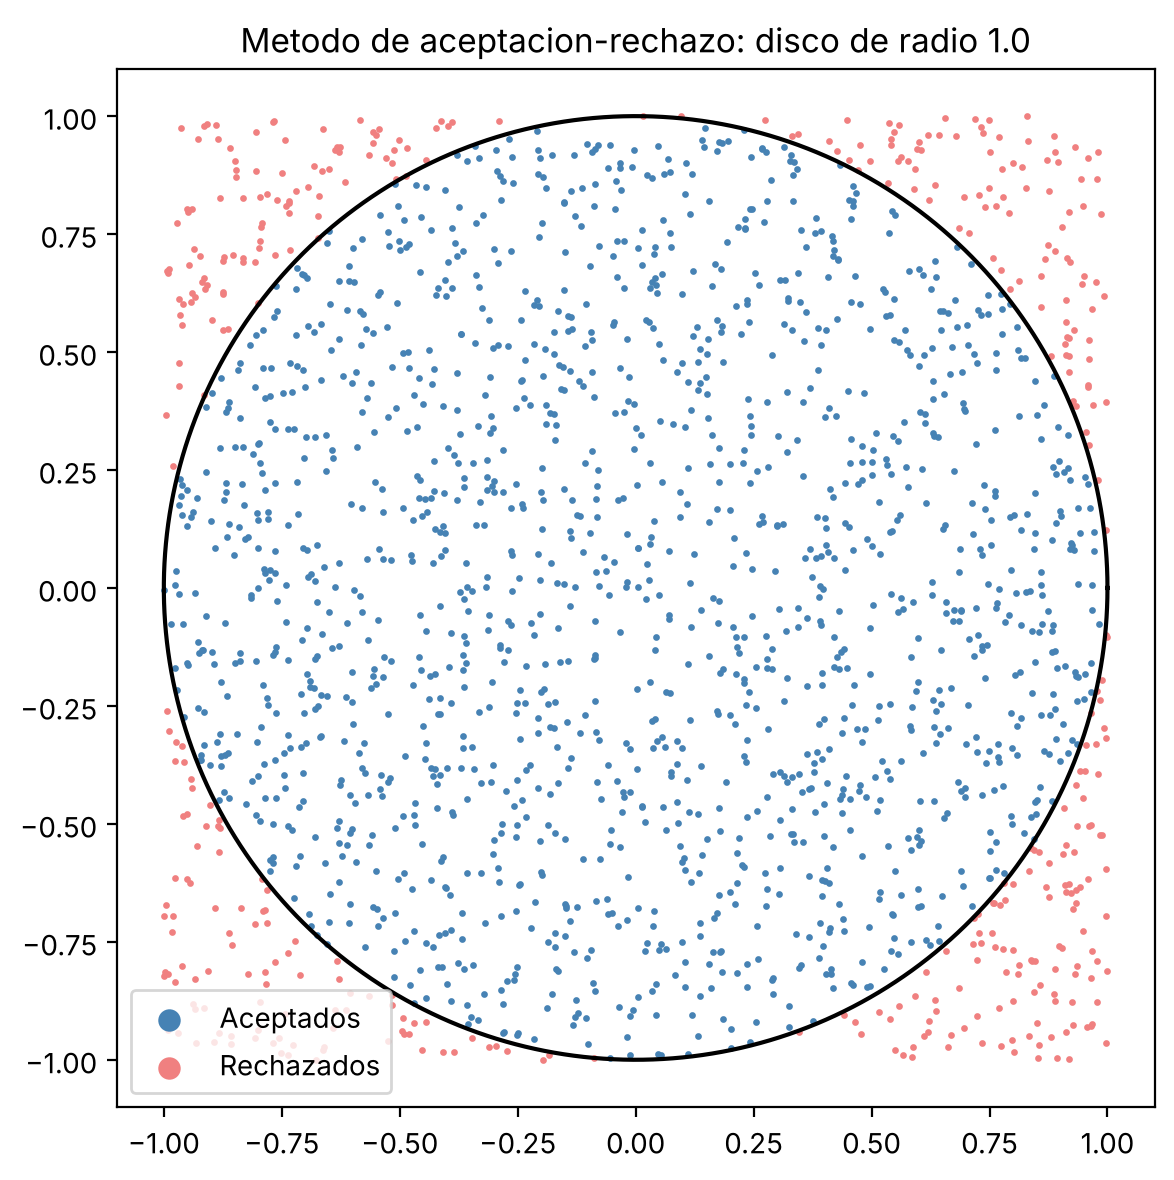
\includegraphics[width=0.5\linewidth]{figs/fig08_disco.png}
\caption{Método de aceptación–rechazo sobre el disco de radio 1: puntos aceptados (azul) y rechazados (rojo).}
\end{figure}

En la visualización, con 2\,000 puntos, la proporción de puntos aceptados es 0,7855, próxima al valor teórico $\pi/4\approx0{,}7854$, lo que proporciona la estimación $\pi\approx3{,}1420$.

\subsection{Comparación con métodos deterministas en 2D}
Se aproxima la misma integral mediante la regla del rectángulo en 2D, evaluando $f$ en los nodos de una malla $m\times m$ sobre $[-r,r]^2$ y sumando únicamente los puntos interiores al disco. Las Tablas~\ref{tab:t12} y~\ref{tab:t13} recogen los resultados.

\begin{table}[H]
\centering
\caption{Regla del rectángulo 2D sobre el disco unitario, con $m$ nodos por dirección.}\label{tab:t12}
\begin{tabular}{cccc}
\toprule
\cab $\boldsymbol{m}$ & \textbf{Evaluaciones} & \textbf{Aproximación} & \textbf{Error}\\
\midrule
10 & 80 & 1,625600 & 0,054804\\
20 & 316 & 1,588600 & 0,017804\\
50 & 1\,976 & 1,590712 & 0,019916\\
100 & 7\,860 & 1,573180 & 0,002384\\
200 & 31\,428 & 1,572002 & 0,001206\\
500 & 196\,364 & 1,571027 & 0,000231\\
\bottomrule
\end{tabular}
\end{table}

\begin{table}[H]
\centering
\caption{Monte Carlo 2D sobre el disco unitario (media de 50 ejecuciones).}\label{tab:t13}
\begin{tabular}{cc}
\toprule
\cab $\boldsymbol{n}$ & \textbf{Error medio}\\
\midrule
100 & 0,077702\\
400 & 0,043126\\
2\,500 & 0,019016\\
10\,000 & 0,006788\\
40\,000 & 0,003933\\
250\,000 & 0,001868\\
\bottomrule
\end{tabular}
\end{table}

\begin{figure}[H]
\centering
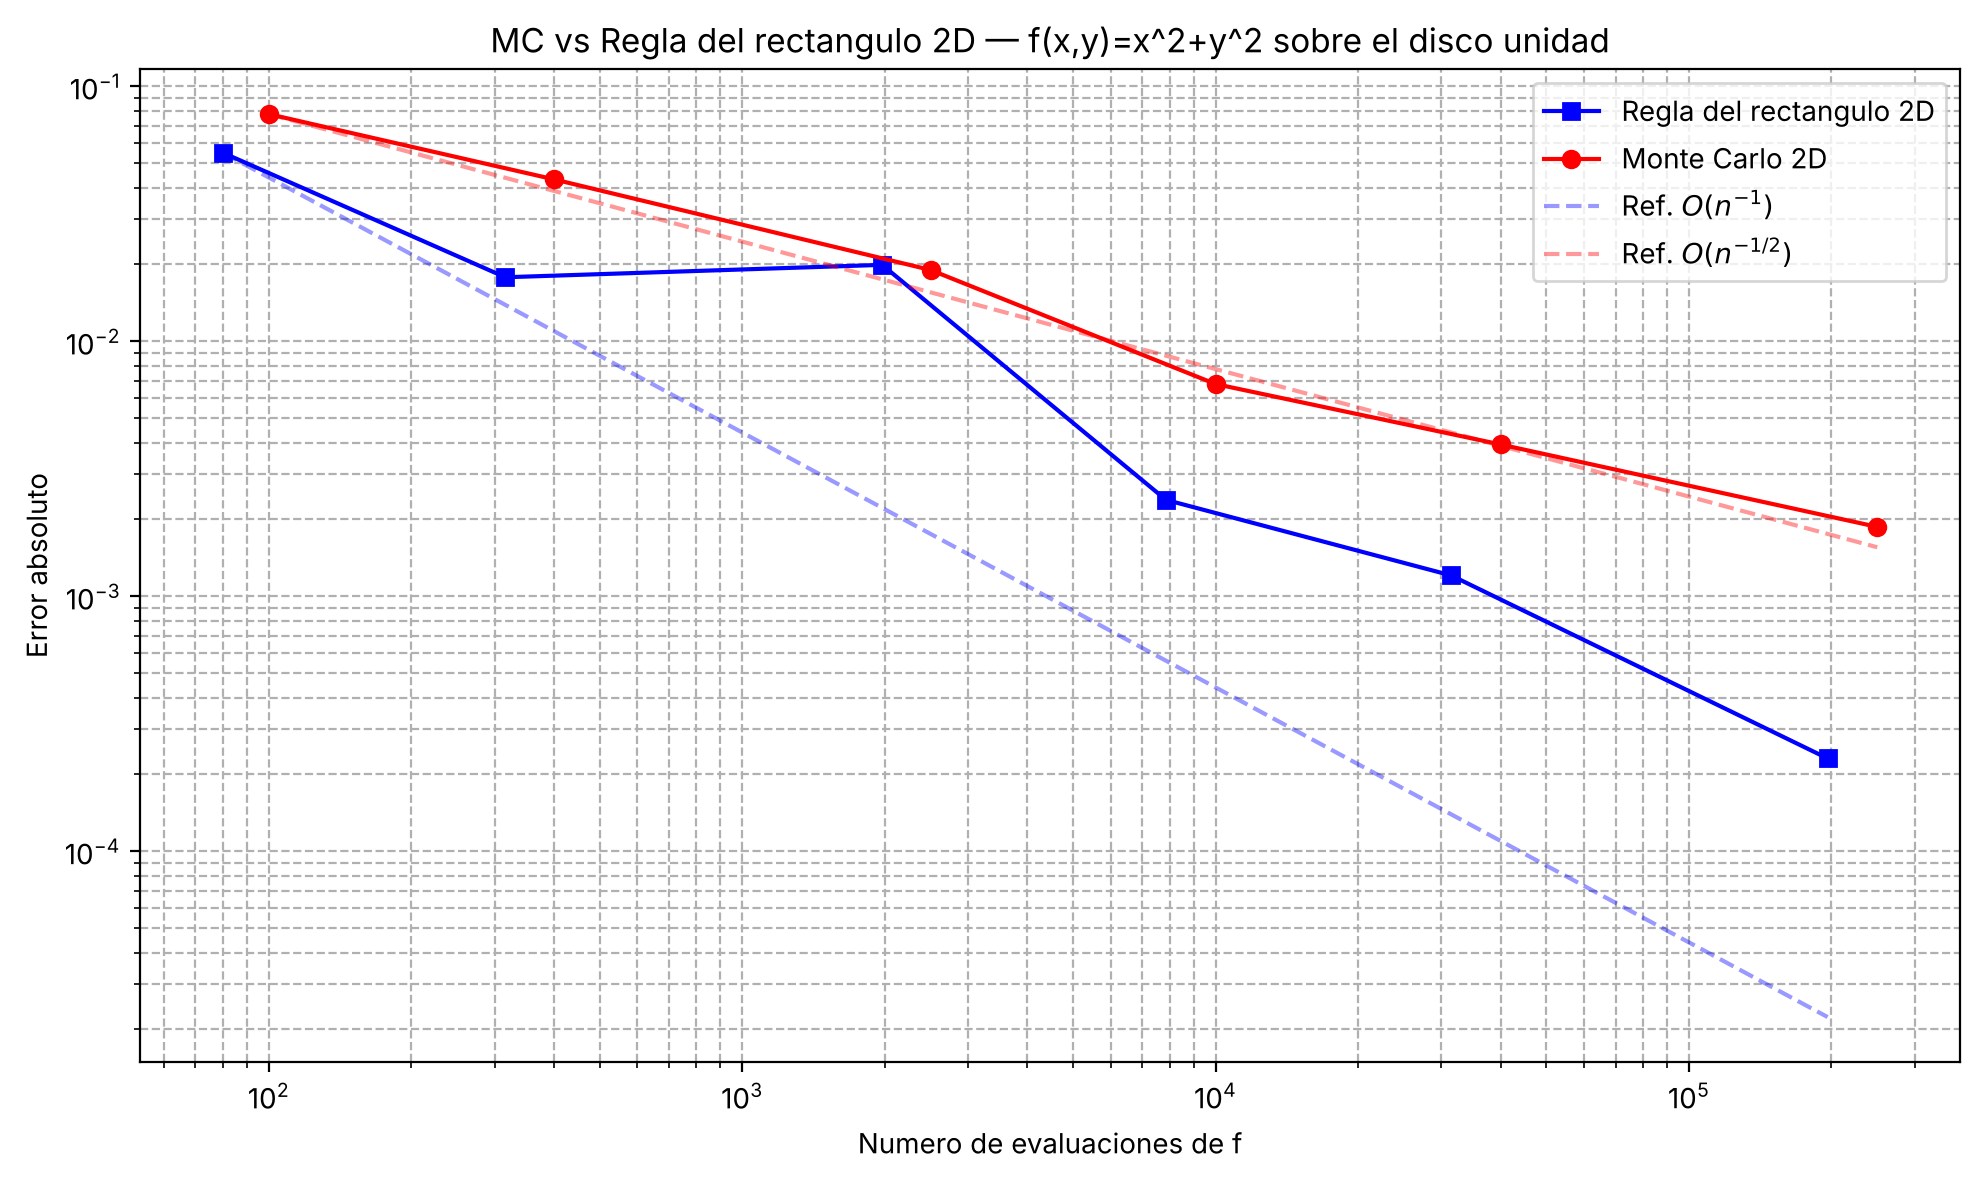
\includegraphics[width=0.8\linewidth]{figs/fig09_disco_rect_vs_mc.png}
\caption{Comparación del error en función del número de evaluaciones para Monte Carlo y regla del rectángulo 2D sobre el disco unidad.}
\end{figure}

Monte Carlo mantiene su orden de convergencia $\mathcal{O}(n^{-1/2})$ en 2D, mientras que la regla del rectángulo converge más lentamente que en 1D, acercándose al comportamiento de Monte Carlo. Este es el primer indicio de la ventaja comparativa que presenta el método al aumentar la dimensión.

\subsection{Dimensión alta}
Se aproxima ahora, mediante Monte Carlo, la integral
\begin{equation}
\int_{[-1,1]^d}\frac{1}{1+\|\mathbf{x}\|_2^{8}}\,\mathrm{d}\mathbf{x}, \qquad \|\mathbf{x}\|_2=\sqrt{x_1^2+x_2^2+\cdots+x_d^2},
\end{equation}
para varios valores de $d$, promediando 20 aproximaciones con $n = 500\,000$. Los resultados se muestran en la Tabla~\ref{tab:t14}.

\begin{table}[H]
\centering
\caption{Aproximación Monte Carlo de la integral en dimensión $d$ con $n = 500\,000$.}\label{tab:t14}
\begin{tabular}{ccc}
\toprule
\cab $\boldsymbol{d}$ & \textbf{Aproximación MC} & \textbf{Desviación típica}\\
\midrule
1 & 1,849296 & 0,000433\\
2 & 2,984461 & 0,001464\\
3 & 4,352186 & 0,002972\\
5 & 7,633527 & 0,010513\\
10 & 22,652040 & 0,048408\\
\bottomrule
\end{tabular}
\end{table}

La función $f(\mathbf{x})=1/(1+\|\mathbf{x}\|_2^8)$ vale casi 1 cerca del origen y tiende a 0 lejos de él. En dimensión alta, casi todo el volumen del hipercubo $[-1,1]^d$ está lejos del origen, por lo que el valor medio de $f$ en el hipercubo (la integral dividida entre su volumen) disminuye con $d$, como recoge la Tabla~\ref{tab:t15}. La integral crece igualmente porque el volumen del hipercubo, $2^d$, aumenta más rápido de lo que disminuye ese valor medio.

\begin{table}[H]
\centering
\caption{Valor medio de $f$ en el hipercubo y desviación típica relativa del estimador, a partir de la Tabla~\ref{tab:t14}.}\label{tab:t15}
\begin{tabular}{cccc}
\toprule
\cab $\boldsymbol{d}$ & \textbf{Volumen $2^d$} & \textbf{Valor medio de $f$} & \textbf{Desv. típica / aproximación}\\
\midrule
1 & 2 & 0,9246 & $2{,}3\cdot10^{-4}$\\
2 & 4 & 0,7461 & $4{,}9\cdot10^{-4}$\\
3 & 8 & 0,5440 & $6{,}8\cdot10^{-4}$\\
5 & 32 & 0,2385 & $1{,}4\cdot10^{-3}$\\
10 & 1\,024 & 0,0221 & $2{,}1\cdot10^{-3}$\\
\bottomrule
\end{tabular}
\end{table}

La desviación típica de las aproximaciones también aumenta con $d$, aunque $n$ sea el mismo en todos los casos, y lo hace incluso en términos relativos. El motivo es que el error de Monte Carlo es aproximadamente
\begin{equation}
\frac{\operatorname{vol}(D)\,\sigma_f}{\sqrt{n}}, \qquad \sigma_f^2=\operatorname{Var}\big[f(\mathbf{X})\big],\quad \mathbf{X}\sim\mathcal{U}(D):
\end{equation}
\noindent el factor $n^{-1/2}$ no depende de la dimensión, pero la constante $\operatorname{vol}(D)\,\sigma_f$ sí. En este caso, al estar $f$ concentrada en una región cada vez más pequeña en proporción al hipercubo, su variabilidad relativa aumenta con $d$.

Al evaluar el coste computacional de ambos métodos en función de $d$ se obtienen los resultados de la Tabla~\ref{tab:t16}. Los tiempos dependen del equipo en el que se ejecuta el código; lo relevante es su evolución con $d$.

\begin{table}[H]
\centering
\caption{Coste computacional comparado: Monte Carlo frente a una malla regular con $m = 10$ nodos por dirección.}\label{tab:t16}
\begin{tabular}{ccccc}
\toprule
\cab $\boldsymbol{d}$ & \textbf{$n$ Monte Carlo} & \textbf{Tiempo MC (s)} & \textbf{$n$ malla $= m^d$} & \textbf{Tiempo malla (s)}\\
\midrule
1 & 100\,000 & 0,0020 & 10 & 0,0002\\
2 & 100\,000 & 0,0044 & 100 & 0,0002\\
3 & 100\,000 & 0,0055 & 1\,000 & 0,0002\\
5 & 100\,000 & 0,0078 & 100\,000 & 0,0061\\
10 & 100\,000 & 0,0138 & 10\,000\,000\,000 & N/A\\
\bottomrule
\end{tabular}
\end{table}

\begin{figure}[H]
\centering
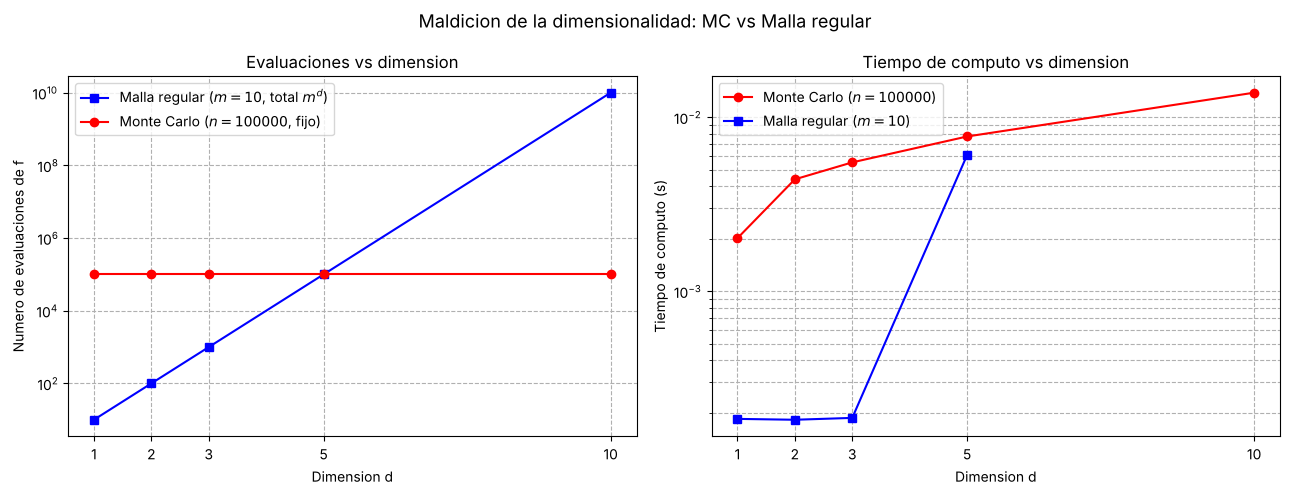
\includegraphics[width=\linewidth]{figs/fig10_dimension.png}
\caption{Maldición de la dimensionalidad: evolución del número de evaluaciones (izquierda) y del tiempo de cómputo (derecha) frente a la dimensión, para Monte Carlo y malla regular.}
\end{figure}

La malla regular requiere $m^d$ evaluaciones, lo que implica un crecimiento exponencial en $d$. Para $m = 10$ y $d = 10$ se necesitarían del orden de $10^{10}$ evaluaciones. En cambio, Monte Carlo utiliza $n$ evaluaciones con un error $\mathcal{O}(n^{-1/2})$, cuyo orden no depende de la dimensión (aunque la constante sí, como se ha visto en la Tabla~\ref{tab:t15}). En dimensión alta, Monte Carlo es la única opción computacionalmente viable, lo que explica su papel central en \emph{Machine Learning} y simulación.

% =================== 9 ===================
\section{Conclusiones}

A lo largo de este proyecto se han estudiado y comparado distintos métodos tipo Monte Carlo para la aproximación de integrales, analizando su variabilidad, su convergencia y su eficiencia frente a los métodos deterministas clásicos.

El método Monte Carlo básico, basado en interpretar la integral como una esperanza y estimarla mediante una media muestral, produce resultados correctos pero con una convergencia lenta, de orden $\mathcal{O}(n^{-1/2})$. Esto implica que reducir el error a la mitad requiere cuadruplicar el número de muestras, lo que lo hace poco competitivo en baja dimensión frente a reglas deterministas como la del rectángulo, cuyo orden es $\mathcal{O}(n^{-1})$, tal y como se ha verificado experimentalmente en las secciones 4 y 7.

La verdadera ventaja de Monte Carlo emerge, sin embargo, en dimensión alta. Mientras que los métodos deterministas basados en mallas requieren un número de evaluaciones que crece exponencialmente con la dimensión ($m^d$), Monte Carlo mantiene su orden de convergencia independientemente de la misma. Este fenómeno, conocido como \emph{maldición de la dimensionalidad}, convierte a los métodos deterministas en inviables a partir de cierta dimensión, como ha quedado de manifiesto en la sección 8.

El método de \emph{importance sampling} ha demostrado ser una mejora significativa del Monte Carlo básico en situaciones en las que la función presenta regiones de alta contribución muy localizadas: picos estrechos, oscilaciones pronunciadas o eventos de baja probabilidad. En la sección 6 se ha comprobado que elegir una densidad propuesta adaptada a la forma de la función reduce notablemente la varianza del estimador, llegando incluso al caso ideal de varianza nula cuando $\rho\propto f$.

En conjunto, el proyecto ilustra el papel dual de los métodos Monte Carlo: relativamente modestos en baja dimensión, donde los métodos clásicos resultan superiores, pero imprescindibles en dimensión alta y en problemas complejos, donde son con frecuencia la única herramienta disponible. Este es precisamente el motivo de su protagonismo en campos como el aprendizaje automático, la física computacional y la ingeniería financiera.

\end{document}
